\section{Case Study}
An example of a real industrial \emph{product detection sorting system} will be shown to explain how the algorithms work.

\subsection{Product Detection Sorting System}
The product detection sorting system is mainly for product quality detecting, as well as sorting. The path delivery facility transmits the product to two conveyors by turns. Both the two conveyors have the \emph{read device} and \emph{write device}, respectively. The read device takes the info from the product to check the quality of the product, and then write the detecting results mark to the product. The sorting section separates the produce by scanning the detecting mark on the product and decide to sort the product into the qualified area or disqualified area.


\subsection{Implement of System Model}
As introduced above, we will describe how to model the system using $IMCL$. The implement of the system model includes three parts:

\textbf{(1) Unifying the resources.} \ \emph{SENSOR} and \emph{DEVICE} are the two types of resource sets where the system can get physical information. The system can get the info from these sensors and control those devices.

\begin{equation*}
\footnotesize
    \begin{aligned}
       & \textbf{SENSOR: }  \{ \ pathSensor, \ sensor1, \ sensor2, \ sortSensor \ \}; \\
       & \textbf{DEVICE: }  \{ \ \emph{PATHSET}, \ \emph{SREAD}1, \ \emph{SWRITE}1, \ \emph{SREAD}2, \ \emph{SWRITE}2, \\
       & \ \ \ \ \ \ \ \ \ \ \ \ \ \ \ \ \emph{SCANNER}, \ \emph{SORTSET} \ \};
    \end{aligned}
\end{equation*}

\begin{figure*}[!htb]
    \centering
        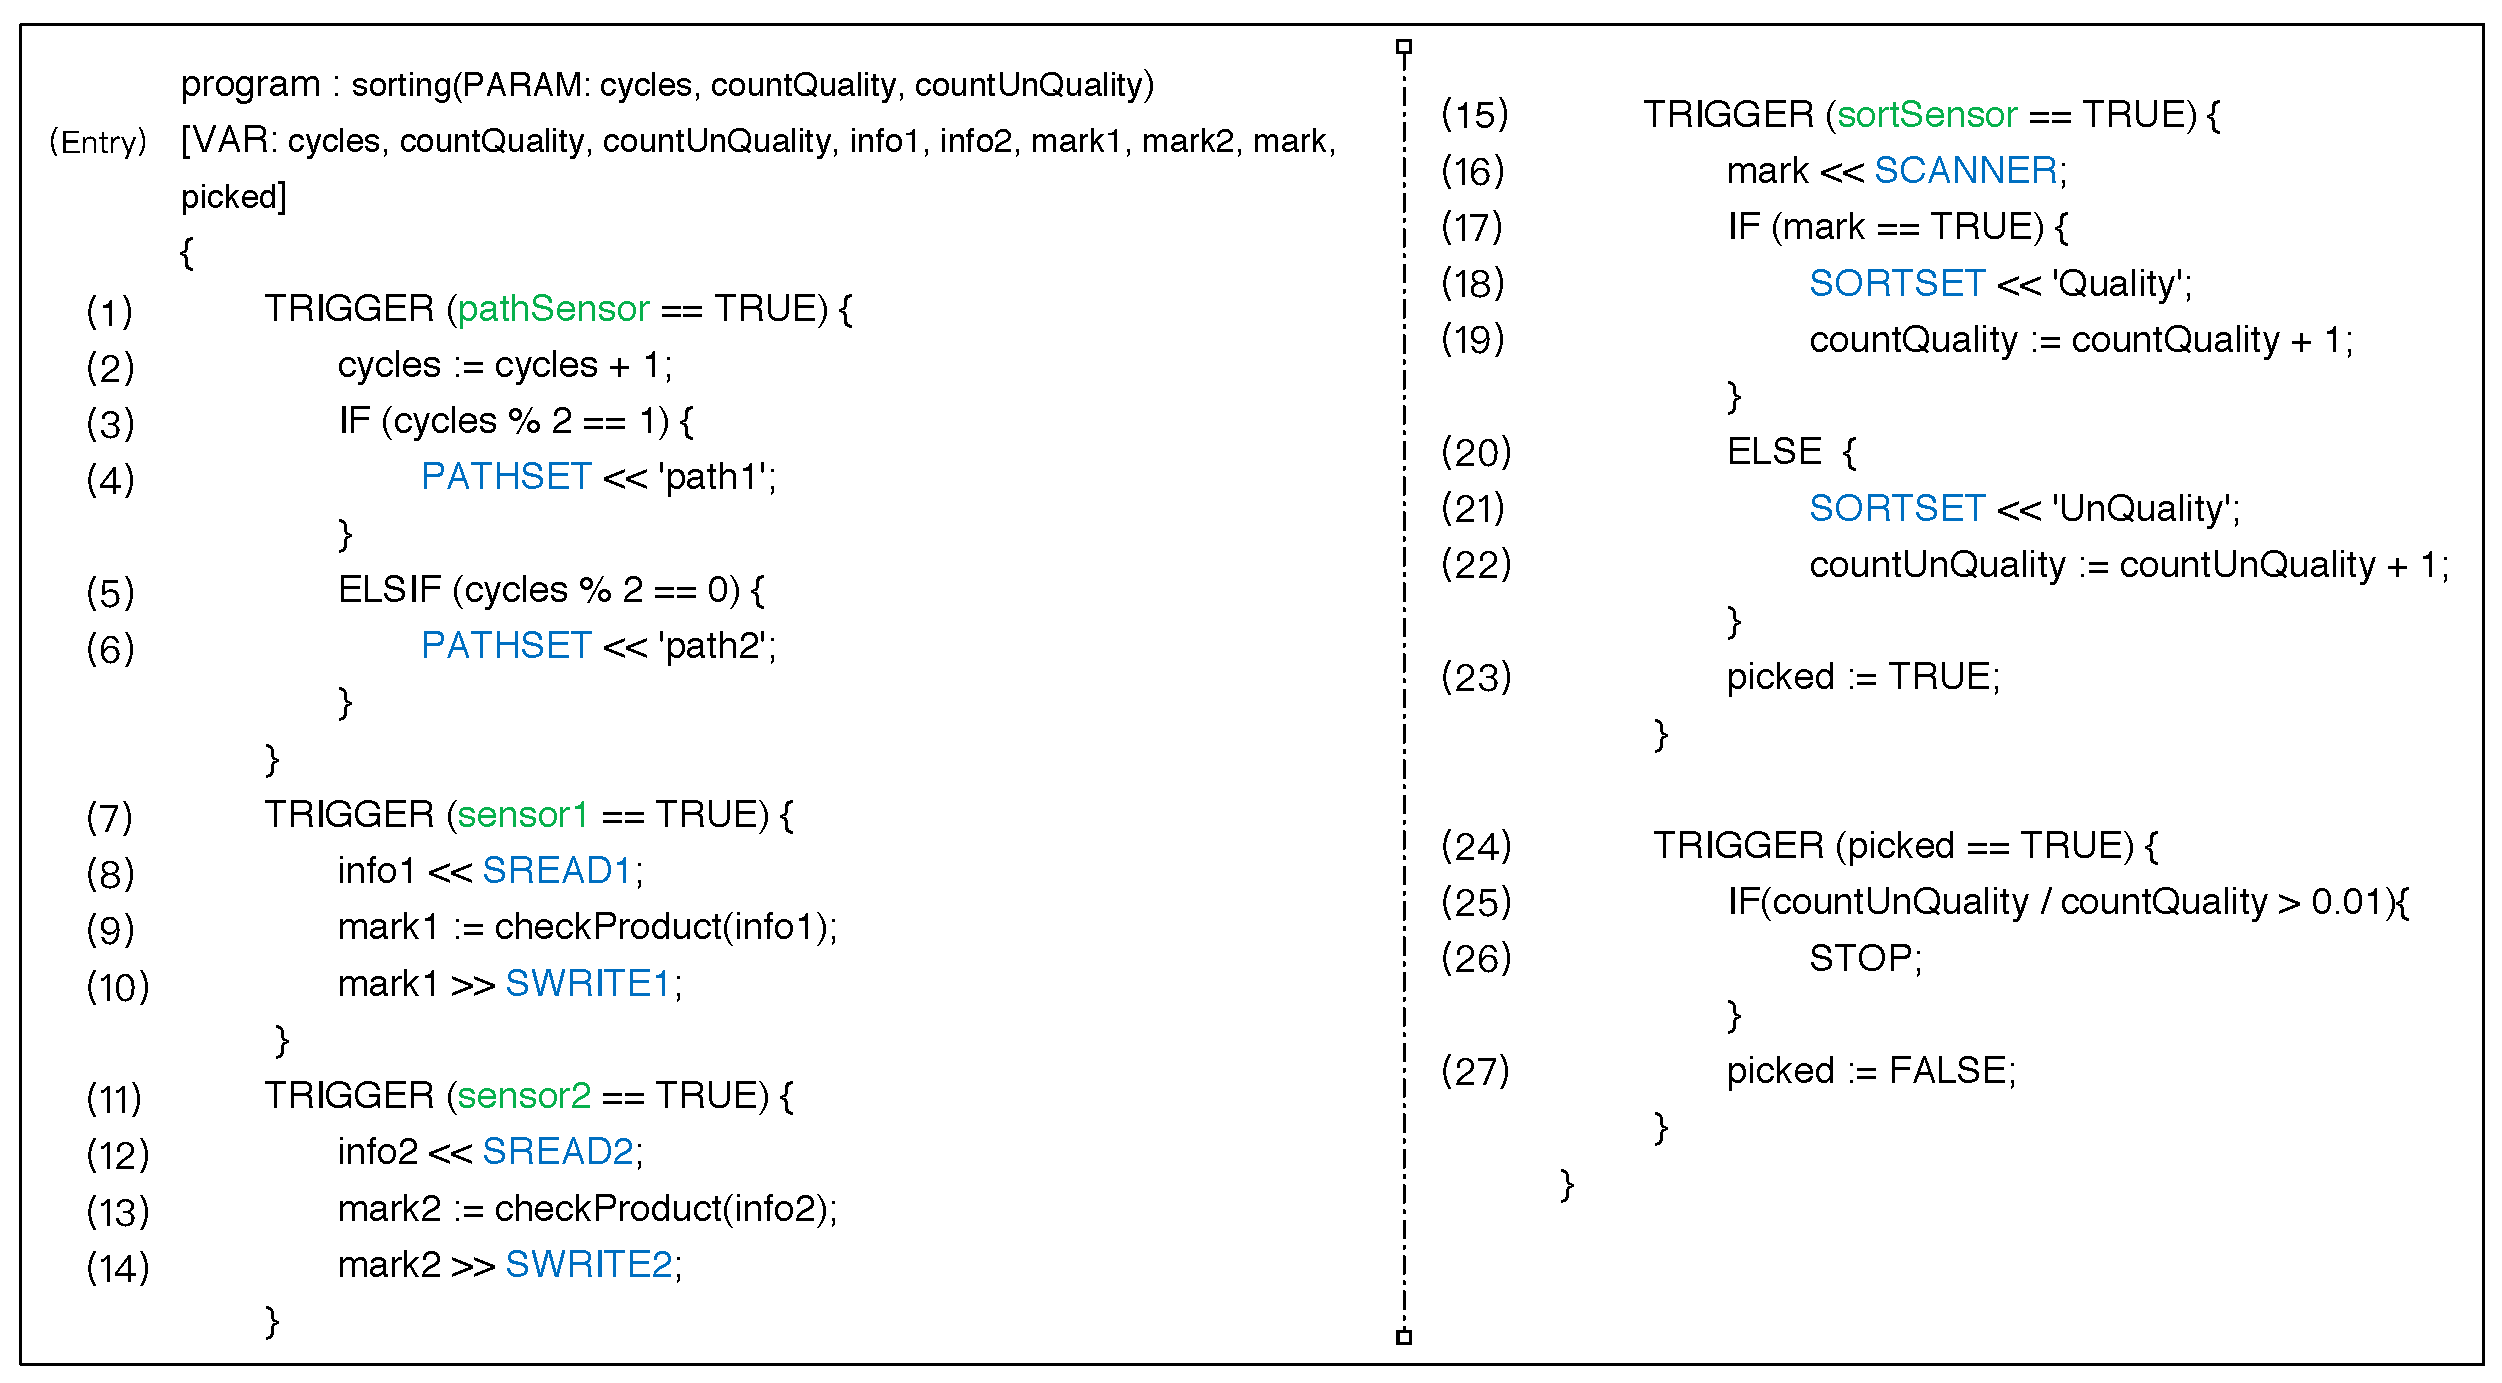
\includegraphics[height=3.0in, width=5.5in]{fig_IMCL_code}
    \caption{Modeling the system using IMCL}\label{fig_IMCL_code}
\end{figure*}

\textbf{(2) Modeling the system.} \ Fig.\ref{fig_IMCL_code} is the \emph{product detection sorting system}. The model contains five event triggers. The first one is triggered when \emph{pathSensor} is true, and \emph{PATHSET} will take a product to the two conveyors. The second one is triggered when the \emph{sensor1} is true; then the \emph{SEAD1} reads the information from the product to check whether it is qualified or not, and then the \emph{SWRITE1} marks the checking result on the product and so does the third event trigger. The fourth one indicates that when the \emph{pathSensor} is true, then the sorting device will determine the sorting of the product by the inspection mark on the product scanned by \emph{SCANNER}. The fifth one indicates that the system checks the system after the \emph{pick} becomes real.



\textbf{(3) Defining resource constraints.} \ The constraints of the resources describe the ability of every \emph{CU}. For example, the computing unit $B_{cu}$ can control two resources \emph{pathSensor} and \emph{PATHSET} in this system model.
\begin{equation*}
\footnotesize
    \begin{aligned}
        \ \textbf{constraint : \ } & \textbf{$A_{cu}$} \ \{ \ \emph{SCANNER}, \ sortSensor, \ \emph{SWRITE}1, \ \emph{SWRITE}2 \ \};\\
        \ \textbf{constraint : \ } & \textbf{$B_{cu}$} \ \{ \ pathSensor, \ \emph{PATHSET} \ \};\\
        \ \textbf{constraint : \ } & \textbf{$C_{cu}$} \ \{ \ sensor1, \ sensor2, \ \emph{SREAD}2, \ \emph{PATHSET} \ \};\\
        \ \textbf{constraint : \ } & \textbf{$D_{cu}$} \ \{ \ \emph{SREAD}1, \ \emph{SWRITE}1, \ \emph{SREAD}2, \ \emph{SORTSET} \ \};
    \end{aligned}
\end{equation*}

\subsection{Decomposition and Collaboration}
Base on the implementation of the model, collaboration model is obtained after decomposing the model with the resource constraints. The whole process consists the resource allocation, decomposition of the model and the collaboration with evaluation.

\textbf{(1) Resource allocation:} \
 \emph{SREAD}2, \emph{SWRITE}1, \emph{PATHSET} are all resource constraints that they can be used by more than one \emph{CU}, and eight solutions of resource constraints would be generated, and are listed in Table \ref{ResourcesAllocation}:

% begin{tabular}{|p{1cm}|p{2cm}|p{3cm}|}
\begin{table*}[!htb]
 \centering
% \tiny\tiny\scriptsize\footnotesize\small\normalsize\large\Large\LARGE\huge\Huge\footnotesize\small\normalsize\large\Large\LARGE\huge\Huge
%\bahao
\small
\caption{\label{ResourcesAllocation}Solutions that CUs are allocated with resources}
\begin{tabular}{|c|c|c|c|c|c|c|c|c|}

\hline

\multirow{2}{*}{\textbf{Resources}} &
\multicolumn{8}{|c|}{CUs allocated with resources ($CU_{\ast}$)} \\
\cline{2-9}
   &\textbf{ Sol 1 } &\textbf{ Sol 2 } &\textbf{ Sol 3 } &\textbf{ Sol 4 } &\textbf{Sol 5 } &\textbf{ Sol 6 } &\textbf{ Sol 7 } &\textbf{ Sol 8 }\\
\hline
\emph{sortSensor}   &$A_{cu}$ &$A_{cu}$ &$A_{cu}$ &$A_{cu}$ &$A_{cu}$ &$A_{cu}$ &$A_{cu}$ &$A_{cu}$ \\
\emph{sensor}2      &$C_{cu}$ &$C_{cu}$ &$C_{cu}$ &$C_{cu}$ &$C_{cu}$ &$C_{cu}$ &$C_{cu}$ &$C_{cu}$ \\
\emph{PATHSET}      &$B_{cu}$ &$C_{cu}$ &$B_{cu}$ &$C_{cu}$ &$B_{cu}$ &$C_{cu}$ &$B_{cu}$ &$C_{cu}$ \\
\emph{SWRITE}1      &$A_{cu}$ &$A_{cu}$ &$D_{cu}$ &$D_{cu}$ &$A_{cu}$ &$A_{cu}$ &$D_{cu}$ &$D_{cu}$ \\
\emph{SWRITE}2      &$A_{cu}$ &$A_{cu}$ &$A_{cu}$ &$A_{cu}$ &$A_{cu}$ &$A_{cu}$ &$A_{cu}$ &$A_{cu}$ \\
\emph{pathSensor}   &$B_{cu}$ &$B_{cu}$ &$B_{cu}$ &$B_{cu}$ &$B_{cu}$ &$B_{cu}$ &$B_{cu}$ &$B_{cu}$ \\
\emph{SORTSET}      &$D_{cu}$ &$D_{cu}$ &$D_{cu}$ &$D_{cu}$ &$D_{cu}$ &$D_{cu}$ &$D_{cu}$ &$D_{cu}$ \\
\emph{SCANNER}      &$A_{cu}$ &$A_{cu}$ &$A_{cu}$ &$A_{cu}$ &$A_{cu}$ &$A_{cu}$ &$A_{cu}$ &$A_{cu}$ \\
\emph{sensor}1      &$C_{cu}$ &$C_{cu}$ &$C_{cu}$ &$C_{cu}$ &$C_{cu}$ &$C_{cu}$ &$C_{cu}$ &$C_{cu}$ \\
\emph{SREAD}1       &$D_{cu}$ &$D_{cu}$ &$D_{cu}$ &$D_{cu}$ &$D_{cu}$ &$D_{cu}$ &$D_{cu}$ &$D_{cu}$ \\
\emph{SREAD}2       &$C_{cu}$ &$C_{cu}$ &$C_{cu}$ &$C_{cu}$ &$D_{cu}$ &$D_{cu}$ &$D_{cu}$ &$D_{cu}$ \\

\hline
\end{tabular}
\end{table*}


% 介绍了不同solution下的不同的分解结果
\textbf{(2) Optimization of Decomposition and Collaboration:} \
There are eight results shown in Table \ref{Evaluations} corresponding to the eight solutions in Table \ref{ResourcesAllocation}.

%\begin{table}[htbp]
\begin{table*}[!htb]
\centering
% \tiny\tiny\scriptsize\footnotesize\small\normalsize\large\Large\LARGE\huge\Huge\footnotesize\small\normalsize\large\Large\LARGE\huge\Huge
\small
\caption{\label{Evaluations}The results of our algorithms for different evaluations}
\begin{tabular}{|c|c|c|c|c|c|c|c|c|}
\hline
\multirow{2}{*}{} &
\multicolumn{4}{|c|}{\textbf{Decompositions}} & \multicolumn{3}{|c|}{\textbf{Collaborations}} &
\multirow{2}{*}{\textbf{Evals}} \\
\cline{2-8}
   &$A_{cu}$ &$B_{cu}$ &$C_{cu}$ &$D_{cu}$ &\emph{ CD } &\emph{ DD } &\emph{SYNC} \\

\hline
\textbf{Sol 1}    &\tabincell{c}{\{ 9,10,13,14,15,16,\\17,19,20,22,23 \}} &\tabincell{c}{\{1,2,3,4,5,6,\\24,25,26,27\}} &\tabincell{c}{\{7,11,12\}} &\tabincell{c}{\{8,18,21\}} &7 &2 &3 &$1.833$ \\
% 0.3*8*8 + 0.4*5*5 + 0.5*1*1 = 29.7
\hline
\textbf{Sol 2}    &\tabincell{c}{\{ 9,10,13,14,15,16,\\17,19,20,22,23 \}} &\tabincell{c}{\{1,2,3,5,24,\\25,26,27\}} &\tabincell{c}{\{4,6,7,\\11,12\}} &\tabincell{c}{\{8,18,21\}} &11 &2 &2 &$2.167$ \\
% 0.3*12*12 + 0.4*5*5 + 0.5*1*1 = 53.7
\hline
\textbf{Sol 3}    &\tabincell{c}{\{ 13,14,15,16,17,\\19,20,22,23 \}} &\tabincell{c}{\{1,2,3,4,5,6,\\24,25,26,27\}} &\tabincell{c}{\{7,11,12\}} &\tabincell{c}{\{8,9,10,\\18,21\}} &\textbf{6} &\textbf{1} &\textbf{2} &\textbf{0.333} \\
% 0.3*7*7 + 0.4*4*4 + 0.5*1*1 = 21.6
\hline
\textbf{Sol 4}    &\tabincell{c}{\{ 13,14,15,16,\\17,19,20,22,23 \}} &\tabincell{c}{\{1,2,3,5,24,\\25,26,27\}} &\tabincell{c}{\{4,6,7,\\11,12\}} &\tabincell{c}{\{8,9,10,\\18,21\}} &10 &1 &2 &$1.0$ \\
% 0.3*11*11 + 0.4*4*4 + 0.5*1*1 = 43.2
\hline
\textbf{Sol 5}    &\tabincell{c}{\{ 1,2,3,4,5,6,\\24,25,26,27 \}} &\tabincell{c}{\{1,2,3,4,5,6,\\24,25,26,27\}} &\tabincell{c}{\{7,11\}} &\tabincell{c}{\{8,12,18,21\}} &8 &2 &2 &$1.667$ \\
% 0.3*8*8 + 0.4*4*4 + 0.5*1*1 = 26.1
\hline
\textbf{Sol 6}    &\tabincell{c}{\{ 9,10,13,14,15,16,\\17,19,20,22,23\}} &\tabincell{c}{\{1,2,3,5,24,\\25,26,27\}} &\tabincell{c}{\{4,6,7,11\}} &\tabincell{c}{\{8,12,18,21\}} &12 &2 &1 &$2.0$ \\
% 0.3*12*12 + 0.4*4*4 + 0.5*1*1 = 50.1
\hline
\textbf{Sol 7}    &\tabincell{c}{\{ 13,14,15,16,17,\\19,20,22,23 \}} &\tabincell{c}{\{1,2,3,4,5,6,\\24,25,26,27\}} &\tabincell{c}{\{7,11\}} &\tabincell{c}{\{8,9,10,\\12,18,21\}} &7 &1 &2 &$1.167$ \\
% 0.3*7*7 + 0.4*3*3 + 0.5*1*1 = 18.8
\hline
\textbf{Sol 8 }    &\tabincell{c}{\{13,14,15,16,17,\\19,20,22,23 \}} &\tabincell{c}{\{1,2,3,5,24,\\25,26,27\}} &\tabincell{c}{\{4,6,7,11\}} &\tabincell{c}{\{8,9,10,\\12,18,21\}} &11 &1 &3 &$1.5$ \\
% 0.3*11*11 + 0.4*3*3 + 0.5*1*1 = 40.4
\hline
\end{tabular}
\end{table*}

\begin{figure*}[!htb]
    \centering
        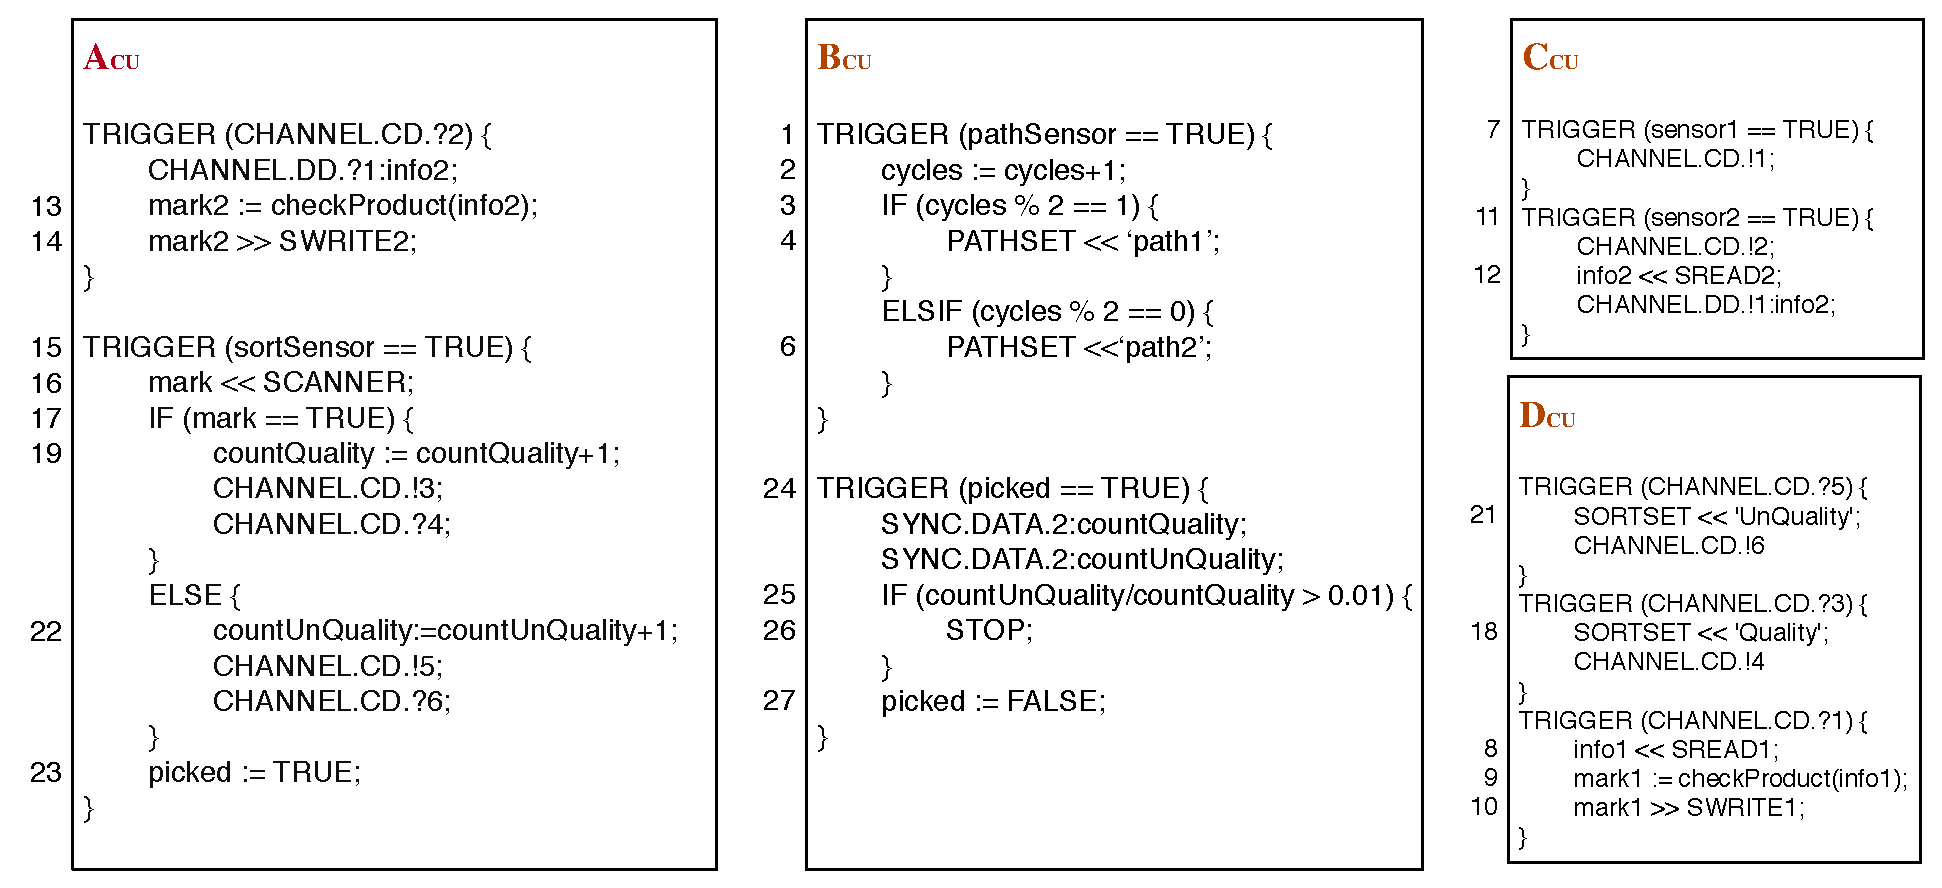
\includegraphics[height=2.7in, width=6.0in]{fig_four_collaborated_program}
    \caption{The collaboration of $A_{cu}$, $B_{cu}$, $C_{cu}$ and $D_{cu}$}\label{fig_four_collaborated_program}
\end{figure*}

As shown in Fig.\ref{fig_IMCL_code}, there are 27 statements in the model that every statement is the minimum computational task level we want to decompose. Table \ref{ResourcesAllocation} shows the eight solutions decomposing the model. In every solution, each \emph{CU} has a set of statements, which means that the \emph{CU} can take the minimum computational tasks in the original model. For example, in \emph{Sol 1}, the $C_{cu}$ decomposed with the set $\{7,11,12\}$, meaning that the $C_{cu}$ are labeled to statement 7, 11 and 12 in sorting system model. The \emph{Collaborations} in this table has three sub-parts: the \emph{CD} shows the number of control dependencies in the collaborative system; the \emph{DD} represents the number of data dependence in the collaborative system; the \emph{SYNC} is the number of data synchronization in the collaborative system. The \emph{Evals} is the evaluation of the collaboration for every solution, and it is the valuation standard of various solutions.
% We set the value \mathrm{}of $w_{cd}$, $w_{dd}$ and $w_{sync}$ in evaluation $Eval$ are $0.3$, $0.4$ and $0.5$ respectively(of course, researcher or developer can assign the value by their actual need).

From the results in Table \ref{Evaluations}, we can conclude that the \emph{Sol} 3 is the most optimizing solution to decompose and collaborate the model. The collaboration of four CUs are shown in Fig.\ref{fig_four_collaborated_program}.

The implementation of this case study can be cloned from our git repository\footnote{http://code.ntesec.com.cn/ju.li/model-slicing.git}.


%\begin{table}[htbp]
%\centering
%\caption{\label{comparison}Result comparison on LN data}
%\begin{tabular}{c|c|c|c|c|c|c|c}
%\hline
%\multirow{2}{*}{Instance} &
%\multirow{2}{*}{Original Instance} &
%\multirow{2}{*}{High Priority} &
%\multirow{2}{*}{Low Priority} &.
%
%\multicolumn{2}{|c|}{Benchmark} & \multicolumn{2}{|c}{Our Algorithm} \\
%\cline{5-8}
%& & & & Utilization & Time(s) & Utilization & Time(s)\\
%\hline
%LN01\&02  &  LN01 \& LN02    &     LN01      &    LN02     &  99.3\%   & 624 &    &   \\
%
%\hline
%\end{tabular}
%\end{table}
%



%\begin{table}[htbp]
%\centering
%\caption{\label{ResourcesAllocation}Result comparison on LN data}
%\begin{tabular}{|c|c|c|c|c|c|c|c|c|c|c|c|}
%\hline
%\scriptsize
%\multirow{2}{*}{Solution} &
%
%
%\multicolumn{11}{|c|}{CUs allocatedwith resources} \\
%\cline{2-12}
%   &\tabincell{c}{path-\\Sensor} &sensor1 &sensor2 &sortSensor &PATHSET &SREAD1 &SWRITE1 &SREAD2 &SWRITE2 &SCANNER &SORTSET \\
%
%\hline
%s0 &s1 &s2 &s3 &s4 &$\backslash$ &r6 &s7 &s8 &r9 &s10 &s11 \\
%s0 &s1 &s2 &s3 &s4 &s5 &r6 &s7 &s8 &r9 &s10 &s11 \\
%s0 &s1 &s2 &s3 &s4 &s5 &r6 &s7 &s8 &r9 &s10 &s11 \\
%
%\hline
%\end{tabular}
%\end{table}

